\documentclass[aspectratio=169,13pt,fleqn] {beamer}
%
% Choose how your presentation looks.
%
% For more themes, color themes and font themes, see:
% http://deic.uab.es/~iblanes/beamer_gallery/index_by_theme.html
%
\mode<presentation>
{
	\usetheme{Madrid}      % 整体主题
	\usecolortheme{beaver} % 配色主题（棕红系）
	\usefonttheme{serif}   % 全局衬线字体（正文宋体类）
	\setbeamertemplate{items}[default] % 【items父模板】控制 itemize+enumerate 符号
%	\setbeamertemplate{items}{\Large\beamertemplateballitem}
	\setbeamertemplate{sections/subsections in toc}[ball] % 目录里章节用圆圈标记
	
	%  \setbeamertemplate{navigation symbols}{} % 取消注释可隐藏底部导航小图标
	\setbeamertemplate{caption}[numbered] % 图/表标题带编号：图1、表1
}

\usepackage[,UTF8,linespread=1.2]{ctex}
\usepackage{wrapfig}
\usepackage{caption}
\usepackage{tcolorbox}
\tcbuselibrary{skins}
\captionsetup[figure]{name=图,labelsep=period}



\usepackage{xcolor}
\definecolor{xy_blue}{cmyk}{0.6,0.35,0.0,0.4}
\definecolor{xy_orange}{cmyk}{0.0,0.7,1.0,0.0}
\definecolor{xy_green}{cmyk}{0.2,0.0,1.0,0.15}
\xdefinecolor{xy_gold}{RGB}{135,103,79}
\xdefinecolor{xy2_gold}{cmyk}{0,0.35,0.75,0.05}

\setbeamercolor{section number projected}{fg=red,bg=red!20}%控制球的颜色
\setbeamercolor{subsection number projected}{fg=blue,bg=blue!40}
\setbeamercolor{item}{fg=xy_gold} %设置列表项颜色

\usepackage{amsthm}
\newtheorem{peroration}{结论：}
\newtheorem*{exploration}{探究：}
\newtheorem*{prooft}{证明：}
\newtheorem*{solve}{解:} 
\newtheorem{instance}{例}   % 解：独立计数器
     

% 配色（你前面需要的，每个环境单独颜色）
\setbeamercolor{theorem}{fg=black,bg=blue!10}
\setbeamercolor{solution}{fg=black,bg=green!10}

\BeforeBeginEnvironment{peroration}{%结论： 
	\setbeamercolor{block title}{bg=xy_green,fg=white}
	\setbeamercolor{block body}{bg=xy_green!10}
}
\AfterEndEnvironment{peroration}{
	\setbeamercolor{block title}{bg=xy_blue,fg=white}
	\setbeamercolor{block body}{bg=xy_blue!10}
}
\BeforeBeginEnvironment{exploration}{%探究
	\setbeamercolor{block title}{bg=xy_orange,fg=white}
	\setbeamercolor{block body}{bg=xy_orange!10}
}
\AfterEndEnvironment{peroration}{
	\setbeamercolor{block title}{bg=xy_blue,fg=white}
	\setbeamercolor{block body}{bg=xy_blue!10}
}
\BeforeBeginEnvironment{solution}{%解
	\begingroup
	\setbeamercolor{block title}{bg=xy_green,fg=white}
	\setbeamercolor{block body}{bg=xy_green!10}
}
\AfterEndEnvironment{solution}{
	\endgroup
}
\BeforeBeginEnvironment{prooft}{%证明
	\setbeamercolor{block title}{bg=xy_green,fg=white}
	\setbeamercolor{block body}{bg=xy_green!10}
}
\AfterEndEnvironment{prooft}{
	\setbeamercolor{block title}{bg=xy_green,fg=white}
	\setbeamercolor{block body}{bg=xy_green!10}
}
\BeforeBeginEnvironment{solve}{%解：
	\setbeamercolor{block title}{bg=xy_orange!60,fg=white}
	\setbeamercolor{block body}{bg=xy_orange!10}
}
\AfterEndEnvironment{solve}{%解：
	\setbeamercolor{block title}{bg=xy_orange!60,fg=white}
	\setbeamercolor{block body}{bg=xy_orange!10}
}
   
\BeforeBeginEnvironment{instance}{% 例子
	\begingroup
   	\setbeamercolor{block title}{bg=xy_gold!40,fg=black}
   	\setbeamercolor{block body}{bg=xy_gold!10}
   }
\AfterEndEnvironment{instance}{
	\endgroup
   }     
   
\renewcommand{\thefigure}{\arabic{figure}}

\title[2.2基本不等式]{2.2~~基本不等式(第3课时)}
\author[好好学习，努力向上]{}
\institute{}
\date{2026.9.24}
\setbeamertemplate{theorems}[numbered]

\AtBeginSection[]
{
  \begin{frame}<beamer>
    \frametitle{本节主要内容}
    \tableofcontents[currentsection,currentsubsection]
  \end{frame}
}

\begin{document}
\begin{frame}{}
	\titlepage
\end{frame}

\begin{frame}{内容概览}
	\tableofcontents
\end{frame}

\section{前情回顾}
\begin{frame}{前情回顾}
	
	\begin{enumerate}[(1)]
		\item 重要不等式：已知$a$、$b\in R$，则
		\[
		\alert{a^2 + b^2 \geqslant 2ab}
		\]
		当且仅当$a=b$时等号成立。
		\item 基本不等式：已知$a$，$b\in R_{\;+}$，则
		\[
		\alert{\sqrt{ab} \leqslant \frac{a+b}{2}}
		\]
		当且仅当$a=b$时等号成立。
	\end{enumerate}
	
\end{frame}

\section{基本不等式的应用}
\begin{frame}[t]{基本不等式的应用1}
	\begin{instance}
		\begin{enumerate}[(\arabic*)]
			\item<1-|alert@1> 用篱笆围一个面积为 $100\ \mathrm{m^2}$ 的矩形菜园，当这个矩形的边长为多少时，所用篱笆最短？最短篱笆的长度是多少？
			\item<2-|alert@2> 用一段长为 $36\ \mathrm{m}$ 的篱笆围成一个矩形菜园，当这个矩形的边长为多少时，菜园的面积最大？最大面积是多少？
		\end{enumerate}
	\end{instance}
	
	
\end{frame}

\begin{frame}[t]{解答...}
\begin{solve}
	设矩形菜园的相邻两条边的长分别为 $x\ \mathrm{m}$，$y\ \mathrm{m}$，篱笆的长度为 $2(x+y)\ \mathrm{m}$。
	\vspace{-1.5em}
	\begin{enumerate}[(1)]
		\begin{columns}[t]
			
		\column{0.48\textwidth}
	\setlength{\itemindent}{2em}
	\item 由已知得 $xy=100$。
	
	由
	\[
	\frac{x+y}{2}\ge \sqrt{xy},
	\]
	可得
	\[
	x+y\ge 2\sqrt{xy}=20,
	\]
	所以
	
		
		
		\column{0.48\textwidth}
		
		\begin{tcolorbox}[blanker,borderline west={2pt}{-30pt}{xy_orange!60},]
			
			\[
			2(x+y)\ge 40,
			\]
			
			
			当且仅当 $x=y=10$ 时，上式等号成立。
			
			因此，当这个矩形菜园是边长为 $10\ \mathrm{m}$ 的正方形时，所用篱笆最短，最短篱笆的长度为 $40\ \mathrm{m}$。
			
			~
		\end{tcolorbox}
		

		\end{columns}
	\end{enumerate}
\end{solve}
\end{frame}

\begin{frame}{解答2...}
	
	\begin{solve}
		\begin{enumerate}[(2)]
		\item 由已知得 $2(x+y)=36$，矩形菜园的面积为 $xy\ \mathrm{m^2}$。
		
		由
		\[
		\sqrt{xy}\le \frac{x+y}{2}=\frac{18}{2}=9,
		\]
		可得
		\[
		xy\le 81,
		\]
		当且仅当 $x=y=9$ 时，上式等号成立。
		
		因此，当这个矩形菜园是边长为 $9\ \mathrm{m}$ 的正方形时，菜园的面积最大，最大面积是 $81\ \mathrm{m^2}$。
		\end{enumerate}
	\end{solve}
\end{frame}
\begin{frame}[t]{基本不等式的应用2}
	\begin{instance}
		某工厂要建造一个长方体形无盖贮水池，其容积为 $4800\ \mathrm{m^3}$，深为 $3\ \mathrm{m}$。如果池底每平方米的造价为 $150$ 元，池壁每平方米的造价为 $120$ 元，那么怎样设计水池能使总造价最低？最低总造价是多少？
	\end{instance}
	\begin{figure}
		\begin{flushright}
			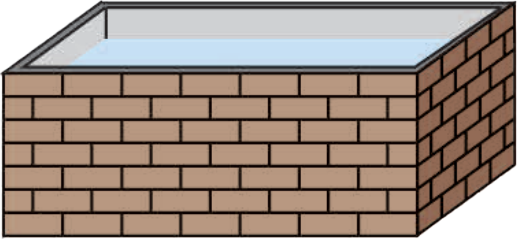
\includegraphics[scale=0.4]{Figures/2026-09-23.png}
		\end{flushright}
		
	\end{figure}	
\end{frame}

\begin{frame}{}
	
	\begin{solve}
		
		\begin{columns}
			\begin{column}{0.45\textwidth}
					设贮水池池底的相邻两条边的边长分别为 $x\ \mathrm{m}$，$y\ \mathrm{m}$，水池的总造价为 $z$ 元。根据题意，有
				\begin{align*}
					z &= 150\times \frac{4800}{3}+120(2\times 3x+2\times 3y) \\
					&= 240\,000+720(x+y).
				\end{align*}
				由容积为 $4800\ \mathrm{m^3}$，可得
				\[
				3xy=4800,
				\]
				因此
			\end{column}
			
			\begin{column}{0.45\textwidth}	
				\begin{tcolorbox}[blanker,%此样式(style) 依赖于empty 皮肤。所有引擎都设置为空(empty)，所有版口(margins) 都设置为0pt。
					frame hidden,
					borderline west={2pt}{-10pt}{xy_orange!60},]
					
					\[
					xy=1600.
					\]
					所以
					\[
					z\ge 240\,000+720\times 2\sqrt{xy},
					\]
					当 $x=y=40$ 时，上式等号成立，此时 $z=297\,600$。
					
					所以，将贮水池的池底设计成边长为 $40\ \mathrm{m}$ 的正方形时总造价最低，最低总造价是 $297\,600$ 元。
				\end{tcolorbox}			
				
			\end{column}
		\end{columns}
	
		
	\end{solve}
\end{frame}




\begin{frame}[t]{布置作业}
	
	P48 练习 ：1--4
	
	P48--49 习题2.2：3--6

\end{frame}

\end{document}
